\documentclass[12pt]{beamer}

\setbeamerfont{block body alerted}{size=\small}

\usetheme{Madrid}
\useoutertheme{shadow}

\usepackage{amsfonts}
\usepackage{hyperref}
\usepackage[super,comma,numbers]{natbib}
\renewcommand{\bibnumfmt}[1]{[#1]}
\bibliographystyle{apsrev4-1}

\title[Annealed model]{More on the annealed model of diffusion in semi-permeable domains}
\author[Hathcock group]{A. Brown | Hathcock group}
\date{January 26, 2026}


\newcommand{\abs}[1]{\left| #1 \right|} % | |
\newcommand{\avg}[1]{\left\langle #1 \right\rangle} % < >


\begin{document}

\maketitle

\begin{frame}{The permeable domain limit}
     \begin{figure}
        \centering
        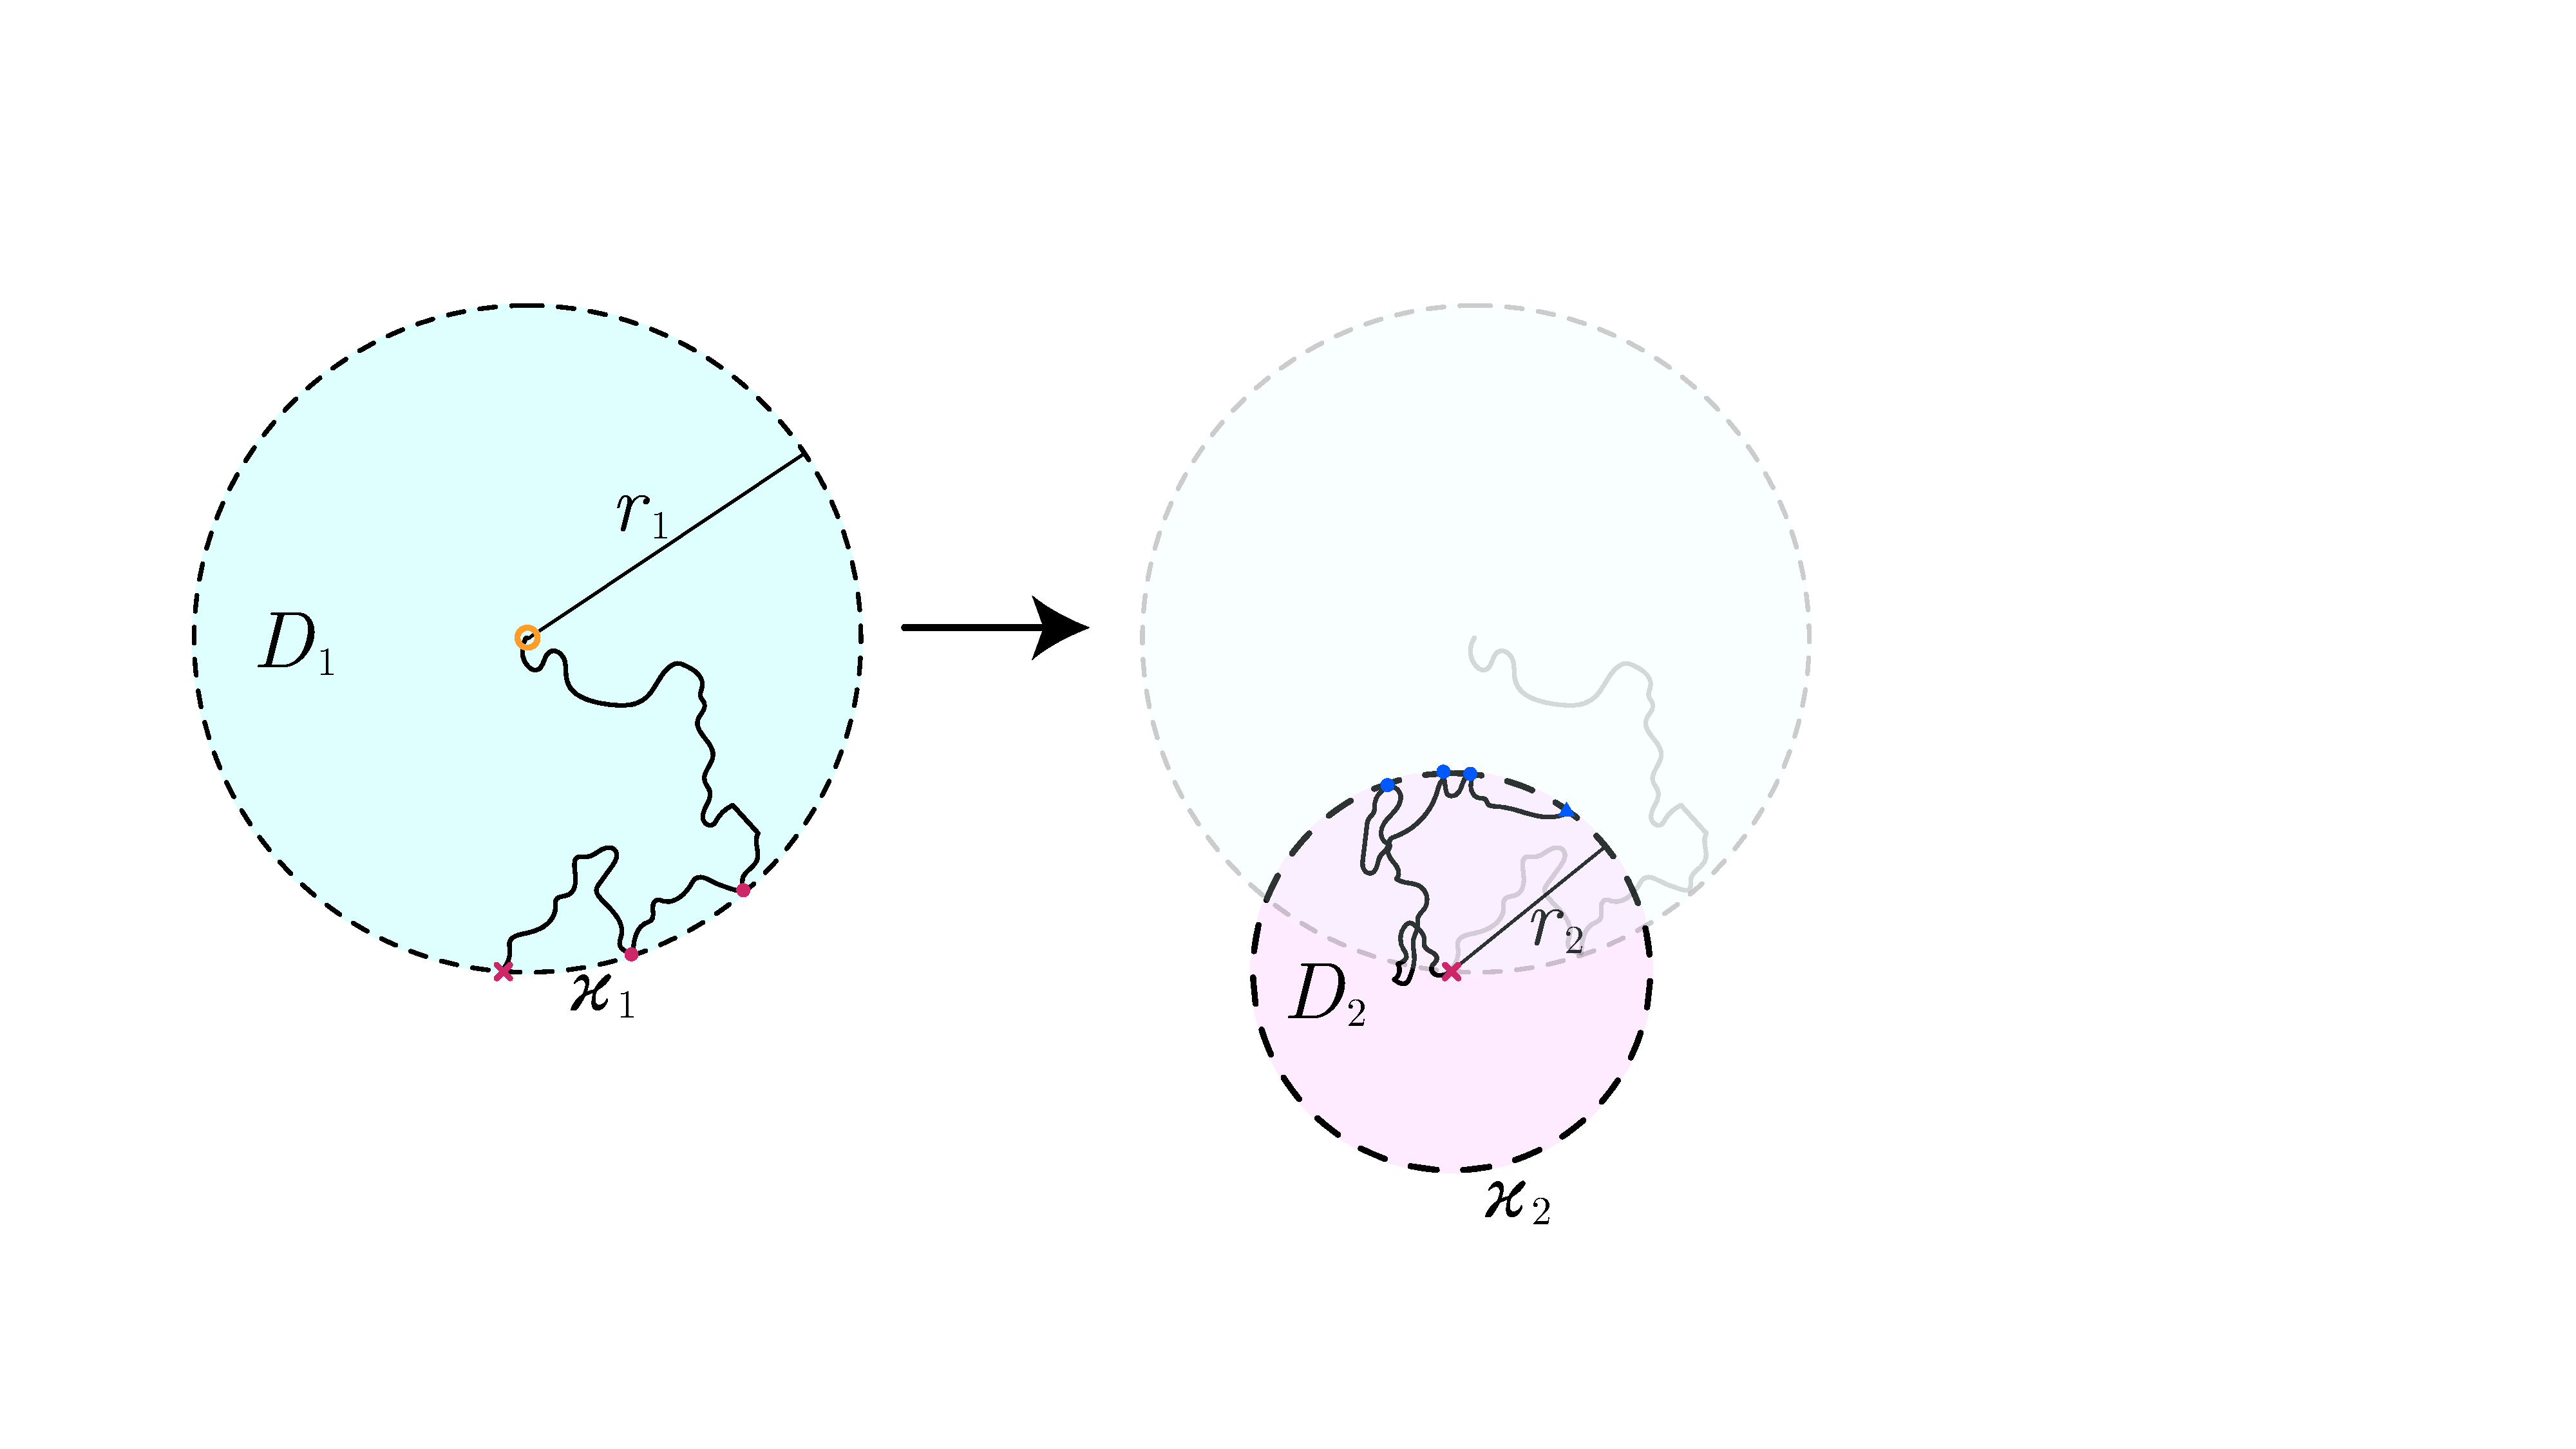
\includegraphics[width=0.65\textwidth]{figures/annealed-model.pdf}
    \end{figure}
    \pause
    \vspace{-6pt}
    \begin{itemize}
        \item Should generically expect that longer steps are penalized by higher time cost~\cite{Oxford.9780199234868.001.0001}
        \begin{itemize}
            \item Necessitates coupling between the position of the walk and time
        \end{itemize}
    \end{itemize}
\end{frame}

\begin{frame}{Joint density}
    \begin{itemize}
        \item Let $\psi(\tau)$ denote the density of the \textbf{patch duration} $\tau$ and
        $\phi(x,t \mid \tau)$ be the propagator for the displacement after
        \textbf{elapsed time} $t\in[0,\tau]$ within that patch.
        We define the joint density
        {%
            \setlength{\belowdisplayskip}{0pt}
            \setlength{\belowdisplayshortskip}{0pt}
            \begin{equation} \label{eq:joint-density}
                \rho (x, t, \tau) = \phi (x, t \mid \tau) \psi (\tau)
            \end{equation}
        }
        \pause
        \item The density of being in an \textbf{unfinished patch} at $(x,t)$ is hence
        {%
            \setlength{\belowdisplayskip}{0pt}
            \setlength{\belowdisplayshortskip}{0pt}
            \begin{equation} \label{eq:unfinished-patch-density}
                \zeta (x, t) = \int_t^\infty \rho (x, t, \tau) \, d \tau
            \end{equation}
        }
        \pause
        \item Let $\eta(x,t)$ be the density of being at $(x,t)$ \textbf{immediately after} a patch completion.
        Then the full propagator $p(x,t)$ is a convolution of renewal points with the unfinished-patch density:
        \begin{equation} \label{eq:convolved-ctrw-propagator}
            p (x,t) = \int_{\mathbb{R}^d} d^d x' \int_0^{t'} dt' \, \eta(x', t') \zeta (x-x', t-t')
        \end{equation}
    \end{itemize}
\end{frame}

\begin{frame}{Fourier-Laplace representation}
    \begin{itemize}
        \item By the convolution theorem applied to Eq.~\eqref{eq:convolved-ctrw-propagator},
        {%
            \setlength{\belowdisplayskip}{0pt}
            \setlength{\belowdisplayshortskip}{0pt}
            \begin{equation} \label{eq:fl-ctrw-propagator-patch}
                \Tilde{p} (k, s) = \Tilde{\eta} (k, s) \Tilde{\zeta} (k, s)
            \end{equation}
        }
        \pause
        \item Patch completions form a renewal process. 
        The renewal density $\eta$ can be written implicitly as
        \begin{equation} \label{eq:patch-completion-density}
            \eta (x, t) = \delta (t) \delta (x) + \int d^d x' \int d t' \, \eta(x', t') w (x - x', t - t')
        \end{equation}
        where $w(x,t)$ is the joint density of \textbf{completed} patch increments (displacement and duration) for one full patch
        \item Completion occurs when $t = \tau$, so
        \begin{equation}\label{eq:completed-kernel}
            w(x,t) = \int_0^\infty d \tau \, \rho(x, t, \tau)
            = \phi(x, t \mid t) \psi(t).
        \end{equation}
    \end{itemize}
\end{frame}

\begin{frame}{Fourier-Laplace propagator}
    \begin{itemize}
        \item Taking the Fourier-Laplace transform of Eq.~\eqref{eq:patch-completion-density} gives
        \[
            \Tilde{\eta} (k, s) = 1 + \Tilde{\eta} (k, s) \Tilde{w} (k, s),
        \]
        hence
        {%
            \setlength{\belowdisplayskip}{0pt}
            \setlength{\belowdisplayshortskip}{0pt}
            \begin{equation} \label{eq:fl-patch-completion-density}
                \Tilde{\eta} (k, s) = \frac{1}{1 - \Tilde{w} (k, s)}
            \end{equation}
        } 
        \pause
        \item Substituting Eq.~\eqref{eq:fl-patch-completion-density} into Eq.~\eqref{eq:fl-ctrw-propagator-patch},
        we get a nice closed form expression for the FL-transformed propagator
        {%
            \setlength{\belowdisplayskip}{0pt}
            \setlength{\belowdisplayshortskip}{0pt}
            \begin{equation} \label{eq:fl-ctrw-propagator-explicit}
                \Tilde{p} (k, s) = \frac{\Tilde{\zeta} (k, s)}{1 - w (k, s)}
            \end{equation}
        }
    \end{itemize}
\end{frame}

\begin{frame}{Fourier-Laplace MSD}
    \begin{itemize}
        \item The transformed propagator $\Tilde{p}$ is the Laplace transform of the characteristic function.
        For an isotropic unbiased process, the Laplace-transformed MSD in $\mathbb{R}^d$ is obtained via the $k$-Laplacian:
        {%
            \setlength{\belowdisplayskip}{0pt}
            \setlength{\belowdisplayshortskip}{0pt}
            \begin{equation} \label{eq:msd-fl-characteristic}
                \avg{\abs{x (s)}^2} = - \left.\Delta_k \Tilde{p}(k,s)\right|_{k=0}
            \end{equation}
        }
        \pause
        \item Differentiating Eq.~\eqref{eq:fl-ctrw-propagator-explicit} and using unbiasedness
        (so $\nabla_k \tilde\zeta(0,s)=\nabla_k \Tilde{w}(0,s)=0$), we obtain
        \begin{equation} \label{eq:msd-fl-explicit}
            \avg{\abs{x (s)}^2} = 
            -\frac{\Delta_k \Tilde{\zeta}(k,s)\big|_{k=0}}{1 - \Tilde{\psi} (s)}
            -\frac{\Delta_k \Tilde{w}(k,s) \big|_{k=0}}{s \bigl( 1 - \Tilde{\psi} (s) \bigr)}.
        \end{equation}
        since $\Tilde{w} (0, s) = \Tilde{\psi} (s)$ and $\Tilde{\zeta}(0,s) = (1 - \Tilde{\psi} (s)) / s$
    \end{itemize}
\end{frame}

\begin{frame}{Reducing to within-patch second moments}
    \begin{itemize}
        \item The remaining inputs in Eq.~\eqref{eq:msd-fl-explicit} are
        $\left.\Delta_k \Tilde{w}(k,s)\right|_{0}$ and $\Delta_k \tilde\zeta(k,s) |_{0}$.
        These can be written entirely in terms of the \textbf{within-patch characteristic function}, $\hat\phi(k,t\mid\tau)$
        \pause
        \item Completion kernel (one full patch):
        {%
            \setlength{\belowdisplayskip}{0pt}
            \setlength{\belowdisplayshortskip}{0pt}
            \begin{equation} \label{eq:laplacian-w}
                \Delta_k \Tilde{w}(0,s)
                = \int_0^\infty dt \, e^{-s t} \psi(t) 
                \left.\Delta_k \hat\phi(k,t\mid t)\right|_{k=0}
            \end{equation}
        }
        \pause
        \item Unfinished-patch kernel:
        {%
            \setlength{\belowdisplayskip}{0pt}
            \setlength{\belowdisplayshortskip}{0pt}
            \begin{equation} \label{eq:laplacian-zeta}
                \Delta_k \Tilde{\zeta}(0,s)
                = \int_0^\infty dt \, e^{-s t} \int_t^\infty d \tau \, \psi(\tau)
                \left.\Delta_k \hat{\phi}(k,t\mid\tau)\right|_{k=0}
            \end{equation}
        }
        \pause
        \item Therefore, determining the MSD reduces to knowing the within-patch MSD
        \[
            M_2 (t \mid \tau) := \int_{\mathbb{R}^d} \abs{x}^2 \phi(x,t\mid\tau) \, d^d x
            = -\left. \Delta_k \hat\phi(k,t\mid\tau) \right|_{k=0}
        \]
    \end{itemize}
\end{frame}

\begin{frame}{Using the patch model}
    \begin{itemize}
        \item The minimum amount of information we can specify is the patch duration density $\psi$ and the within-patch MSD $M_2$
        \pause
        \item For now, let's specify the full within-patch propagator itself.
        For Brownian motion on a patch with (possibly $\tau$-dependent) diffusivity $D(\tau)$,~\cite{PhysRevLett.112.150603}
        {%
            \setlength{\belowdisplayskip}{0pt}
            \setlength{\belowdisplayshortskip}{0pt}
            \begin{equation} \label{eq:bm-propagator}
                \phi (x, t \mid \tau) = \frac{1}{(4 \pi D (\tau) t)^{d/2}} \exp{\left( - \frac{x^2}{4 D (\tau) t} \right)},
                \qquad t \leq \tau
            \end{equation}
        }
        \pause
        \begin{itemize}
            \item Its spatial F.T. is Gaussian: $\hat{\phi}(k, t \mid \tau) = e^{-D (\tau) k^2 t}$.
            Consequently, $M_2 (t \mid \tau) = -\Delta_k \hat{\phi}(k, t \mid \tau)|_{k=0} = 2d D(\tau) t$
            \pause
            \item For fractional Brownian motion within a patch one analogously has
            $M_2(t\mid\tau)=2d K_{\beta}(\tau) t^{\beta}$,
            where $K_{\beta}(\tau)$ is the generalized diffusion coefficient on a patch.
        \end{itemize}
    \end{itemize}
\end{frame}

\begin{frame}{Tauberian theorems}
    \begin{itemize}
        \item Suppose we are to follow the main text and let $\psi (\tau) \sim \tau^{- \alpha - 1}$ and $D \sim \tau^{-1/\gamma}$.
        For Brownian motion, the Laplacian of the Fourier transform can be read off from Eq.~\eqref{eq:laplacian-w}
        {%   
            \setlength{\belowdisplayskip}{0pt}
            \setlength{\belowdisplayshortskip}{0pt}
            \[
                - \Delta_k \Tilde{w} (0,s) \sim 2 d \int_0^\infty d t \, e^{- s t} t^{- \rho}, \qquad \rho = \alpha + 1/\gamma
            \]
        }
        \pause
        \begin{itemize}
            \item Issue: this integral only converges when $\Re{(\rho)} < 1$
            \pause
            \item Can determine its asymptotic properties more generally via the 
            Tauberian theorem~\cite{Feller.Probability2}: Let $f(t)$ be a real-valued function of bounded variation.
            For $\rho \in (0,1)$, the following statements are equivalent of $f$ and its Laplace transform $F$,
            \begin{equation} \label{eq:tauberian-theorem}
                F(s) \sim s^{-\rho}, \quad s \to 0; \qquad 
                f(t) \sim t^{\rho-1} / \Gamma(\rho), \quad t \to \infty
            \end{equation} 
        \end{itemize}
    \end{itemize}
\end{frame}

\begin{frame}{Applications of the Tauberian theorems I}
    \begin{itemize}
        \item Since $\psi$ is a probability distribution function, it permits the 
        asymptotic expansion via the Tauberian theorems~\cite{Feller.Probability2}
        {%
            \setlength{\belowdisplayskip}{0pt}
            \setlength{\belowdisplayshortskip}{0pt}
            \begin{equation} \label{eq:asymptotic-laplace-patch-duration}
                \Tilde{\psi} (s) \sim 1 - c s^\alpha + o(s^\alpha), \qquad s \to 0
            \end{equation}
        }
        \pause
        \item If $\rho = \alpha + 1 / \gamma <1$, we can calculate the transforms in the numerators explicitly~\cite{Bateman.Integrals1},
        \[
            - \left. \Delta_k \Tilde{w} (k,s) \right|_{k = 0} \sim s^{\rho-1}, \qquad
            - \left. \Delta_k \Tilde{\zeta} (k,s) \right|_{k = 0} \sim s^{\rho-2}
        \]
        so both terms in Eq.~\eqref{eq:msd-fl-explicit} give rise to the same exponent,
        \begin{equation} \label{eq:casei-msd}
            \avg{\abs{x (s)}^2} \sim s^{-2+1/\gamma} \quad \implies \quad
            \avg{\abs{x (t)}^2} \sim t^{1-1/\gamma},
        \end{equation}
        via an inversion Tauberian of the Tauberian theorem
    \end{itemize}
\end{frame}

\begin{frame}{Applications of the Tauberian theorems II}
    \begin{itemize}
        \item On the other hand, when $\rho > 1$, the integral decays sufficiently fast at infinity 
        such that the limit exists and is finite,
        {%
            \setlength{\belowdisplayskip}{0pt}
            \setlength{\belowdisplayshortskip}{0pt}
            \begin{equation} \label{eq:w-limit-large-w}
                -\Delta_k \tilde w(k,s)\big|_{k=0} \; \xrightarrow[s\to 0]{} \;
                C_w:=\int_0^\infty \psi(t)M_2(t\mid t)\,dt
            \end{equation}
        }
        \pause
        \item Meanwhile $1-\tilde\psi(s)\sim c\,s^\alpha$ still holds.
        Insert \eqref{eq:w-limit-large-w} into Eq.~\eqref{eq:msd-fl-explicit}:
        the second term behaves as
        {%
            \setlength{\belowdisplayskip}{0pt}
            \setlength{\belowdisplayshortskip}{0pt}
            \[
                \frac{-\Delta_k \tilde w|_{0}}{s\,(1-\tilde\psi(s))}
                \sim \frac{C_w}{s \times c s^\alpha}
                = \text{const.} \times s^{-1-\alpha}.
            \]
        }
        \pause
        \item A similar piece of argumentation follows for the second term.
        Completing a Tauberian inversion we find
        {%
            \setlength{\belowdisplayskip}{0pt}
            \setlength{\belowdisplayshortskip}{0pt}
            \begin{equation} \label{eq:caseii-msd}
                \avg{\abs{x (s)}^2} \sim s^{-1-\alpha} \quad \implies \quad
                \avg{\abs{x (t)}^2} \sim t^{\alpha},
            \end{equation}
        }
    \end{itemize}
\end{frame}

\begin{frame}{What about FBM?}
    \begin{itemize}
        \item If the within-patch motion is instead that of FBM with $K_\beta (\tau) \sim \tau^{-1/\gamma}$,
        for $\delta = \alpha + \frac{1}{\gamma} + 1 - \beta < 1$,
        \begin{equation} \label{eq:casei-msd-fbm}
            \avg{\abs{x (t)}^2} \sim t^{\beta-1/\gamma}
        \end{equation}
        and subsequently for $\delta > 1$, the analysis remains the same as above and is dominated by the waiting time,
        \begin{equation}\label{eq:caseii-msd-fbm}
            \avg{\abs{x (t)}^2} \sim t^{\alpha}.
        \end{equation}
        \pause
        \item FBM and per-patch scaling of diffusivity can obscure each other!
    \end{itemize}
\end{frame}


% \begin{equation} \label{eq:fl-bm-propagator}
%     \Tilde{\phi} (k, t \mid t) = \sum_{n = 0}^\infty \frac{(-1)^n k^{2n}}{n!} 
%     \frac{\Gamma ((1 - \gamma)n + 1)}{s^{(1 - \gamma)n + 1}}
% \end{equation}

\begin{frame}{References}
    \bibliography{references}
\end{frame}

\begin{frame}{Fourier-Laplace notation}
    Throughout, the Laplace transform of a function $f(t)$ is written
    \begin{equation} \label{eq:laplace-transform}
        F (s) = \int_0^\infty dt \, e^{-s t} f (t)
    \end{equation}
    Likewise, the Fourier transform of a function $f(x)$ is written
    \begin{equation} \label{eq:fourier-transform}
        \hat{f} (k) = \int d^d x \, e^{- i k \cdot x} f(x)
    \end{equation}
    and its inverse transform
    \begin{equation} \label{eq:inverse-fourier-transform}
        f(x) = \int \frac{d^d k}{(2 \pi)^d} \, e^{i k \cdot x} \hat{f} (k)
    \end{equation}
\end{frame}

\begin{frame}{Laplace transform of an ``exponential power law''}
    Consider the function
    \[
        f(t) = e^{- a t^w},
    \]
    for constants $a > 0, \Re{(w)} > -1$.
    Our interest lies in its Laplace transform, as defined in Eq.~\eqref{eq:laplace-transform}.
    We can expand the exponential as a power series,
    \[
        e^{- a t^w} = \sum_{n = 0}^\infty \frac{(-1)^n}{n!} a^n t^{wn}
    \]
    and use the identity~\cite{Bateman.Integrals1}
    \[
        \int_0^\infty e^{- s t} t^\nu \, dt = \frac{\Gamma (\nu + 1)}{s^{\nu + 1}},
    \]
    for $\Re{\nu} > -1$, we can write the transform as a power series,
    \begin{equation}
        F (s) = \sum_{n = 0}^\infty \frac{(-1)^n a^n}{n!} \frac{\Gamma (wn + 1)}{s^{wn + 1}}
    \end{equation}
\end{frame}

\end{document}